%\pagestyle{article}
\documentclass[a4paper]{article}
\usepackage[english]{babel}
\usepackage[utf8]{inputenc}
\usepackage{graphicx} % for figures
\usepackage[section]{placeins} %This prevents placing floats before a section.
\usepackage{csquotes}

\usepackage{natbib}% better citation
\usepackage{hyperref} %autoref
\usepackage{amsmath} % for \tag and \eqref macros in mathematical eq.

%% Sets linestretch, paragraphstrech, indentation and footnote stuff 
\usepackage{parskip} %space between paragraphs
\parskip=12pt %set space between paragraphs
\setlength\parindent{12pt} %paragraf indentation
\usepackage[onehalfspacing]{setspace} %linespacing; does not affect footnotes
\setlength{\footnotesep}{0.7\baselineskip}% space between footnotes
\usepackage[hang,flushmargin]{footmisc} %% removes identation in footnoteshttps://www.overleaf.com/project/5b98e00a21d3bd15ac5a2e86

\usepackage{makecell} % make cells in tabels for longer text

\usepackage[colorinlistoftodos]{todonotes}

%% For header and footer (1)
% Marco
\usepackage{fancyhdr}
\pagestyle{fancy}
\textwidth = 424pt % test width ish
\oddsidemargin = 18pt % margin width ish

\fancyheadoffset{0 in} % Shifty solutions..

\fancyhf{} %% clear defuelt header and footer

%% For header and footer (2)
%Specifics
\lhead{Simon P. von der Maase}
\rhead{\today}

\lfoot{University of Copenhagen}
\rfoot{\thepage}
\renewcommand{\footrulewidth}{0.8pt}

\title{A Morden Approach to Conflict Prediction\\or: Dude, Here's Your Conflict\\ or: Where Men Rebel}

\author{Simon Polichinel von der Maase}
\date{September 2018}

\begin{document}

	\begin{titlepage}
		\maketitle
		\noindent\rule{\linewidth}{0.4pt}
		\begin{figure}[h]
			\centering
			
\includegraphics[scale=0.32]{KU_logo.png}
		\end{figure}
		\thispagestyle{empty} % removes page number on front page
	\end{titlepage}
    \tableofcontents
\pagebreak

\begin{abstract}
\todo[inline]{To come..}
\end{abstract}
\pagebreak

\section{Introduction}
%\subsection{The 'What'}

% Du har ikke data med fra efter 2010 fordi den igen der bliver for ufuldstændig..

Humans kill humans - a lot of humans. In 2009 an estimated 46,772 people were killed in internal conflicts alone\footnote{according to the best estimate from the Uppsala Conflict Data Program}. The number of lives ruined as a consequence of these killings no doubt exceeds the number of deaths by magnitudes. Even far away from the conflict zones people experiences the consequences of conflict - not least in the form of large influx of refugees and the ensuring political turmoil. The long term solution to this senseless onslaught probably entails some fundamental changes to the global power structures involving the cooperation of the global political, economic and cultural elites alike. However, while we wait for this eventuality to ensue, another, less Utopian approach would be to mitigate the ongoing catastrophe by creating a reliable "early warning system". A predictive framework capable of estimating the probability that a given geographic location will experience conflict during a given time period. Using this information governments, NGOs or other responsive actors can act to prevent the conflict, mitigate the fallout, or secure civilians. Naturally, such interventions are both disruptive and expensive. Thus, for any predictive framework to work as a practical early-warning-system a high level of accuracy is needed; we need to ensure that the geographic locations, which are being appointed the highest risk by the framework, are indeed where future conflicts are most likely to occur.\par

This paper presents a modern computational approach to conflict prediction and forecasting. It is constructed as a unified framework to asses the probability that a given sub-national geographical location will experience battle-related deaths as a consequence of intra-state conflict. The challenge is handled as a forecasting problem, thus the prediction target is whether or not the given location experiences any battle-related deaths \emph{"next year"}.\par 

This is a preliminary project, thus the aim is as much to explore fruitful approaches and methods for future research as it is making good predictions. As a consequence, the larger part of this paper is dedicated to choosing what goes into the model and not least evaluating what comes out.\par

What goes in to the model is a roster of features derived from both the theoretical and empirical literature regarding civil wars and intra-state conflict. What comes out of the model, is first of all probabilities of conflict deaths pertaining to a given geographical cell in a given year; which are then evaluated against the actual observations. But just as importantly, the framework allows for evaluation of the individual feature's importance in the prediction process. This insight is paramount in deciding how to improve the framework and where to invest resources in future endeavours.\par

The framework constructed shows great promise; out-of-sample prediction generally estimates high probability of conflicts where conflicts actually ensues. One challenge is that the framework still has a hard time separating very close and similar cells from each other leading to some lack in precision. That is, if we where to classify all cells with a probability of conflict above 10\% as future conflict zones, we capture almost 80\% percent of all future conflicts; however, we would also classify two false positives for each true positive. While these cells are mostly adjacent, it still means, that we will have a hard time pinpointing the exact cell. Furthermore, the model struggles to capture sudden political developments such as peace agreements, and would not fare well predicting new conflict-onsets far removed from any other conflicts in time and space.\par

Going forward with future endeavours I recommend allocating resources to create a more unified and systematic framework modeling the temporal-spatial evolution of conflicts as a function of it self. For one thing, it seems the most productive way to improve prediction power as features pertaining these dimensions contributed with nearly all the prediction power in the present framework. Secondly, but just as important, the conflict data is more frequently updated and the last entry is closer to the present year then the contextual features used in this project.\par

Another source of more up-to-data and topical data could be text data from news sources or political outlets. This might also amend the framework's inability to capture novel political developments.\par

The following subsections will first present the motivation followed by the research questions and design. Then, a short presentation of the included features. Next I present the predictive framework and a thorough analysis of the derived results. This is proceeded by a discussion regarding future challenges and suggestions for improvements. Lastly a conclusion sums up the main findings.\par

\subsection{The 'Why'}

\begin{displayquote}
\emph{[...] the estate of Man can never be without some incommodity or other; and [...] the greatest, that in any form of Government can possibly happen to the people in generall, is scarce sensible, in respect of the miseries, and horrible calamities, that accompany a Civill Warre;} \cite[128]{Hobbes_1991} \par

\end{displayquote}

The perils and miseries of civil war and internal conflict have plagued mankind all throughout history - not least in modern times. Since the conclusion of the Second World War intra-state conflicts have been far more common than inter-state wars \citep[563]{Collier_Hoeffler_2004}; Over five times as many people have died in intra-state conflicts compared to inter-state wars \citep[563]{Collier_Hoeffler_2004}; and since 1960 over one half of all nations have experienced some sort of violent internal conflict leading to fatalities \citep[3-4]{Blattman_Miguel_2010}.\par

Importantly, Internal conflicts should not be viewed as internal affairs of little concern to other then the inflicted host and its allied. Examples of spillover-effects facilitating the spread of conflicts across boarders a ample. At country level, having a country located in a conflict ridden neighbourhood have been shown to be a robust predictor of internal conflict \citep{Hegre_Sambanis_2006,Goldstone_2010}. Internal conflict is thus a highly destructive and potentially contentious malaise. Understanding how internal conflicts originates and spreads in order to prevent or mitigate the destruction is indeed as crucial as ever.\par

Encouragingly, developments in statistical techniques, data availability and computational power makes the endeavour slightly more feasible with each passing year \footnote{Unless, of course, conflict is inherently shrouded in ontological uncertainty rather than epidemiological uncertainty as implied by \cite{Gartzke_1999}}. One recent development is the shift in focus from cross country comparison towards disaggregated analyzes on sub-country unites. Given the nature of intra-state conflicts, this development is a promising step towards a better understanding of the phenomenon \citep{Cederman_Gleditsch_2009}. The disaggregated approach is further enhanced by evermore accessible geospatial software and powerful new machine learning algorithms. As I will show, these developments can aid us in the construction of a reliable early-warning-system.\par

\subsection{The 'How'}

The endeavour at hand can be summed up by three research questions:\par

\textbf{$\textrm{First research question} (Q_{1})$:} To what extent\footnote{The phrase "To what extent [...]" present in $Q_1$ implies the caveat: " - Given the scope of the project and the limited computational resources at my disposal. As this is preliminary research I will spend more time evaluating the results and discussing how to improve future frameworks than I will training and fine-tuning the model and optimizing hyper parameters.} is it possible to predict the geographic location of future intra-state conflicts using a modern computational approach.\par

\textbf{$\textrm{Second research question} (Q_{2})$:} What phenomenons and features presents themselves as the most important in this prediction effort.\par

\textbf{$\textrm{Third research question} (Q_{3})$:} Given the conclusions pertaining to $Q_1$ and $Q_2$ what can be done to create an even more informative feature space in the future.\par

To answer these questions I use data from the Uppsala Conflict Data Program (UCDP) \citep{Sundberg_2013, Croicu_Sundberg_2017}. This data includes counts of conflict related deaths along with both coordinates of the scene and estimated time of the event. The coordinates are linked up to specific geographical cells of $0.5 \times 0.5$ decimal degrees derived from the PRIO grid database \citep{Tollefsen_2012}. I aggregate the conflict data to sum up the yearly number of conflict deaths in a given cell. This measure is further dichotomized such that it only indicates whether or not a given cell experienced conflict deaths or not. I then "lead" the measure, effectively lagging all explanatory features to come. Or put another way; I shift the target feature one year ahead (t+1) such that the explanatory features of e.g. 2006 will try to predict conflicts in 2007. Thus, when I further down write "at year = t" I mean the year \emph{preceding} the prediction. To further mimic the forecasting nature of the problem, the model is created only on the basis of data from 1990 through to 2005. Data from 2006 to 2010 are reserved for model evaluation through out-of-sample prediction.\par

To create the explanatory features I borrow from both the Uppsala conflict data itself and from the large number of features available from the PRIO grid database. To mitigate overfitting, secure robustness and aid in the quest of new insights, I constrain myself to create features which corresponds to theoretical salient phenomenons described in the larger literature on civil wars and internal conflicts. I do not demand the connection to be causal; it can be spurious as long as it comes before the conflict in time, and that spurious link is theoretically meaningful. The aim is purely to predict conflict - not explain it. Due to limitation in the available data from the PRIO grid database, the date only covers 1990 through 2010. This is naturally a big obstacle if the framework was ever to be applied in practice, and as such, I shall return to this challenge in the discussion. Further description of the data sources can be found in the appendix, \autoref{data_sources}.\par

With target and features in place, I construct a predictive framework using an ensemble of xgboost algorithms. I use a large ensemble to generate a more robust result and to facilitate insights into the uncertainty inherent in the prediction effort. For robustness, I construct both a model including all observations and one only including new "cell-onsets".\par

The next section will present the features derived from the data sources briefly introduced above.\par

\section{The Included Features}

In this section I will introduce the roster of features used in the endeavour at hand. Some features are readily available from one of the two data sources, other requires some feature engineering before they correspond to the theoretical phenomenon believed to be related to internal conflicts. I draw on insights from both the country aggregated civil war literature and the more resent disaggregated conflict litterateur. As such, some features are cell specific, while others are country specific, and yet others denotes the difference between cell and country values. While it would be satisfying to present the features through a comprehensive literature review, thus also presenting the theoretical justification, the scope and focus of this endeavour does not allow such academic gluttony\footnote{Readings which, together, serve as a rather comprehensive review are \cite{Hegre_Sambanis_2006}, \cite{Kalyvas_2007}, \cite{Cederman_Gleditsch_2009} and \cite{Blattman_Miguel_2010}}. The appendix, \autoref{feature_expanded} presents slightly more comprehensive theoretical justifications and background context for all features below along relevant mathematical definitions. Here, in the main text the reader will have to settle for the following overview:\par

% det sidste over stående stykke kan fjernes hvis du ikke magter dit appendix.

\paragraph{Wealth and Capacities:} Reflecting the various arguments regarding wealth as a conflict inhibitor as put forth in \cite{Collier_Hoeffler_1998, Fearon_Laitin_2003, Collier_Hoeffler_2004}. Here, however, with light night emission as a proxy for wealth, as proposed by \cite{Elvidge_2009}, \cite{Chen_Nordhuas_2011} and \cite{Cederman_Gleditsch_Buhaug_2013}. I have included both a cell-specific and country specific measures, both divided by the population count of the specific country/cell.\par

\paragraph{Inequality and deprivation:} Reflecting the argument concerning relative deprivation as a facilitator of conflict as put forth by \cite{Gurr_1970} and revitalized by \cite{Cederman_Gleditsch_Buhaug_2013}. Here, I also utilize night light emission as a proxy for wealth and I included both the specific measure used in \cite{Cederman_Gleditsch_Buhaug_2013} and a more simple measure simply capturing whether or not a given cell is less wealthy compared to the median cell of the corresponding country.\par

\paragraph{Ethnicity and Exclusion:} A dichotomous feature denoting whether or not the cell is inhabited by one or more excluded ethnic groups (e.i. discriminated or politically powerless) at any given year. This captures the argumentation put forth in \cite{Cederman_Weidmann_Gleditsch_2011, Cederman_Gleditsch_Buhaug_2013}\footnote{the measures are originally from the GeoEPR/EPR data by \cite{Vogt_2015}}.\par

\paragraph{Population size and density:} The correlation between the size of a country's population and the risk of civil war has been found rather robust \citep{Collier_Hoeffler_1998, Fearon_Laitin_2003, Collier_Hoeffler_2004, Hegre_Sambanis_2006}. Furthermore \cite[287]{Fearon_2004} also finds that country population is correlated with longer civil wars. I include measures of both absolute\footnote{Density and logged was tried but yielded no better results} population counts for both cell and country.\par 

\paragraph{Geography and Accessibility:} \cite{Fearon_Laitin_2003} argue that rough terrain and mountains are natural obstacles hindering effective projection of state power. \cite{Hegre_Sambanis_2006} conclude, that a feature for rough terrain is found to be robustly positively correlated with civil war across a large number of model specifications.\cite[526-529]{Hegre_Sambanis_2006}\footnote{Though, see \cite{Goldstone_2010}}. The PRIO grid includes a readily available feature measuring the proportion of mountainous terrain within the cell\footnote{based on \cite{Blyth_2002}} which I utilize.\par

\paragraph{Distance to Power Center:} Another natural hindering for projecting state power is sheer distance \citep{Fearon_2004, Buhaug_Gates_Lujala_2009, Cederman_Buhaug_Roed_2009, Buhaug_2010}. To capture phenomenons like this I have included the distance to the nation's capital\footnote{The measure utilized by \cite{Buhaug_2010}}, the travel time to the nearest major city, and the total size of the country \citep{prio_code_2015}.\par

\paragraph{Trans-boarder Influences:} A number of different mechanism have been proposed and explored \citep[29-30]{Blattman_Miguel_2010}, the one explored here is rather simple and follows \cite{Hegre_Sambanis_2006}. This is simply the distance to the nearest (land) boarder shared with another country.\par 

\paragraph{Prime Commodities, Oil and the Recourse course:} A lot have been written on this subject, but the empirical results have varied a lot \citep{Collier_Hoeffler_1998, Fearon_Laitin_2003, Fearon_2004, Ross_2004, Collier_Hoeffler_2004, Fearon_2005, Buhaug_2010, Hegre_Oestby_Raleigh_2009}. In this endeavour, I include a dichotomous feature denoting whether or not a given cell is known to hold oil deposits. Thus, a cell is not denoted as having oil before oil is actually discovered.\par

\paragraph{Inertia, dispersion, traps and time trends:} Conflict traps and inertia have been modelled or proposed by \cite{Collier_Hoeffler_2004}, \cite{Hegre_Sambanis_2006}, \cite{perry_2013} and \cite{Cederman_Gleditsch_Buhaug_2013} while cross-country dispersion has been used by \cite{Goldstone_2010}. I include a number of features which aims to capture the pattern of conflict as it moves through space and time. Distance from cell center to nearest conflict, yearly fatalities in cell, yearly fatalities in the country as a whole and the total number of years the given cell has been a conflict zone in the past and .\par

As already noted, the features are measured at $year = t$, with the target at $year = t+1$. Thus, when I e.g. define "distance from cell center to nearest conflict", the measure concerns the year preceding the actual prediction.\par

A lot more features and specifications were applied and tested\footnote{Not least logged variants and various density measures. See the appendix, \autoref{feature_expanded}} and even more could have been scrutinized. Furthermore some of the included features could be even better specified. Never-the-less, the features presented above will do for now. I now proceed to presenting the model, the estimations and the results.

\section{The Predictive Framework and the Results}

In the follow sections I present the predictive framework and evaluate the performance of the framework through various metrics. One of the greater challenges pertaining to the project at hand is the imbalance of the data; most of the time, most grid cells do not experience any conflict fatalities. The data as such is imbalanced and only around 1\% of the data constitutes "events" - actual conflicts. I take a number of steps in order to handle imbalanced data: I use a suitable estimation procedure, I under-sample the non-events and I utilize the appropriate evaluation metrics. These approaches will all be presented in the sections below.\par

But first, I will briefly highlight some of the main difference between a dedicated prediction efforts such as this endeavour, and the parameter estimations that many scholars of social and political science are accustomed to.\par

\subsection{Parameter Estimation vs. Prediction}

Most scholars of political and social science are familiar with the process of estimating parameters through e.g. linear or logistic regression. Often the main concern in these efforts is to ensure that the parameter estimates are 'unbiased'; that parameters derived represent the true relationship between the dependent and independent variables under scrutiny. The endeavour at hand takes a different focus; predicting future events. The framework produces no parameters to evaluate, I do not include or exclude features on basis on some statistical significance level and I do not overly concern my self with bias. Instead I concern myself mainly with increasing prediction power and preventing "over-fitting". Indeed traditional models for parameter estimates are perfectly capable of making predictions, but these predictions are often rather poor not least do to overfitting \citep{Ward_Greenhill_Bakke_2010}. Overfitting, to put it simply, is the accidental identification of patterns present in the data, yet not present as a phenomenon in the real world \citep[166-168]{Mcelreath_2018}. In quantitative studies of conflicts scholars have often neglected taking steps to counter overfitting leading to bad estimations and possible erroneous conclusions \citep{king_zeng_2001b, Ward_Greenhill_Bakke_2010}.\par

Preventing overfitting is paramount if I am to generate reliable predictions for real world applications. One tool available is using out-of-sample prediction as evaluation approach \citep{king_zeng_2001b, Ward_Greenhill_Bakke_2010, perry_2013, Schrodt_2014}. This simply entails construction the predictive framework on one set of data and testing it on another; a training set and a test set. Now, if the model fits well on in-sample data but poorly on out-of-sample data, we know that we overfitted the framework to the training data. While out-of-sample predictions can give an honest evaluation and reveal overfitting, other tools are needed to mitigate and prevent the problem in the first place. Some of these I shall return to shortly.\par

A conventional ratio is between 25/75 and 30/70 for test- and training set respectively \citep{Friedman_2001, Ward_Greenhill_Bakke_2010}. I use a ratio of roughly 25/75. To further mimic the forecasting element of the project I choose the last years of the data as the test set and the fist years as the training set \citep{Goldstone_2010}. Thus, years from 1990 through 2005 constitutes my training set and the years including 2006 through 2010 constitutes my test set.\par

I shall return to how exactly to evaluate the out-of-sample performance of the framework further down. However, in the next section I will first introduce the predictive framework it self.\par

\subsection{Predictive Framework}

Having outlined the fundamentals of predictions I now turn to the framework it self. The predictive framework is made up by a subset of approaches. The subsections below present each step at a time, before moving on to the evaluation effort in the next section.\par

\subsubsection{Extreme Gradient Boosting}

I utilize the Extreme Gradient Boosting (xgboost) algorithm as the basis of my predictions \citep{Chen_2016}\footnote{Implemented through python}. This method is a bit advanced and as such I shall refrain from digging too deep into the technicalities of the algorithm. However, some fundamentals serve to explain why this framework is especially well suited for the problem at hand. Three characteristics are especially worth presenting; it is a boosting algorithm, it is consisting of regression trees and it is self-regularizing (or self-pruning).

Boosting involves using a lot of weak classifiers to create a strong classifier. Imagine that we begin with one classifier with which we try to classify geographic locations which will experience conflict fatalities next year. The classifier does rather poorly, not least due to the fact that the events are few and and hard to classify. Thus, we decide to run a new classifier, but now we give less weight to the observations which was correctly predicted and more weight to the observations which was incorrectly predicted. We reiterate this procedure until some measurement criteria is met. Then, all our classifiers are weighted according to their performance and used as a weighted ensemble to predict which geographic locations will experience conflict fatalities of the following year \citep[338-339]{Friedman_2001}. Since the procedure ensures continuing focus on "hard to classify" observations, it is a particularly fruitfully approach when dealing with imbalanced data.\par

The Next question is naturally which classifiers to build our boosting framework on. Xgboost utilizes regression tree. These closely resembles decision tress where the features are used to split the observations into categories according to which splits yields the most information according to some predefined criteria. Thus, the first split would here be the split which best sorted conflict events from non-events and so on. But unlike decision trees, each regression tree holds a continuous score on each of the leafs, which can be converted into probabilities rather then binary classifications \citep[2]{Chen_2016}. To put it simply, xgboost utilizes N number of regression tress and iteratively uses the predictions of one tree to update the weights of the next tree, such that 'harder to classify' observations are given continuously more and more attention.\par

The last question here is then how to decide to number of times we shall allow a given tree to split. Too few times and the tree fails to learn any pattern of the data and we underfit. To many splits and the tree starts to learn idiosyncratic artifacts of the training data and we overfit. The xgboost algorithm handles this by penalizing complicated tress. Thus, when the algorithm evaluates whether or not to make a split, the information gain obtained by the potential split is down-weighted according to the increased complexity induced by new splits \cite[4-7]{Chen_2016}. Thus, the algorithm searches for any patterns which might help the prediction effort, but stops before such pattern becomes overly complicated.\par 

Naturally there is more to the xgboost algorithm than presented here, not least the fact that it has been optimized for sparse data in a number of more technical ways making it even more suited for large and imbalanced data-set then other boosting algorithms \cite[5]{Chen_2016}. Furthermore, the algorithm has a plethora of hyper parameters which can be tuned and optimized to further enhance performance and reduce overfitting\footnote{Usually optimized using k-fold cross validation \citep[241-249]{Friedman_2001}}. This is beyond the scope of this project however, and while it would probably increase the predictive power of the framework somewhat, it would change nothing in regards to the overall approach or the challenges going forward.\par 

Thus, while the complexity is great and the opportunities many, the small introduction above will suffice to illustrate why the approach works well for the problem at hand but also why, as we shall see, there still are some challenges ahead.\par

A final note on the xgboost algorithm pertains to an important property induced by the approach being based on regression trees: one can readily asses how "important" each included feature is in the prediction effort. Given the exploratory nature of the present endeavour it is paramount that I am able to evaluate which features might present the most fertile research areas in future prediction efforts.\par

\subsubsection{Undersampling}

While the boosting approach presented above is able to handle imbalanced problems, we can help it along by re-sampling our training data to create a more balanced ratio between events and non-events. This is called undersampling \citep[1266-1267]{He_2008}. Different variants of this approach have been proposed as a general solution to the imbalance often challenges statistical research on international relations and conflict studies \cite{King_Zeng_2001, king_zeng_2001b}. The specific procedure employed here is called case-cohort sampling. Here, one utilizes all available events from the training set along a random subset of no-events from the training set in order to construct the classifiers used \citep[142]{King_Zeng_2001}. Some trial and error showed that around 20 times as many non-events as events yielded the best prediction results. This means that instead of events being 1\% of the training data, events now constitute around 5\% of the training data. Not a big difference, but enough to do the trick. The actual probabilities estimates are, however, inflated since the model thinks that conflicts are less rare than is the actually the case; this is corrected using Bayesian prior correction closely related to what is presented in \cite{King_Zeng_2001, king_zeng_2001b} and \cite{Goldstone_2010}. The procedure is trivial and are presented in the appendix, \autoref{bayes_correction}. Suffice it to say it corrects the estimated probabilities according to the true propensity of internal conflicts. As I refrain from setting any final hard threshold regarding when a predicted probability should manifest into an actual conflict, this correction does not change the overall performance of the framework; it merely presents the estimated probabilities in a more intuitively appealing and honest light.\par

Returning to the task at hand; while most of the information in the data is stored in the events and not the non-events \cite[139]{King_Zeng_2001}, some information is still lost by not using all non-events. The chosen solution is to utilize a variant of 'informed undersampling'. To counter the inefficient use of information, one can use an ensemble of classifiers all utilizing a new independent subset of non-events to combine with the subset of all available events \cite[1267]{He_2008}. This approach not only utilizes all information available, but also facilities the estimation of the uncertainty inherent in the prediction effort. That is, not only do I get an estimated probability, I also get an estimate of how reliable that probability is. The practical steps are simple; I run the same xgboost classifier 1000 times using a new independent subset of non-events drawn from the training set along all events present in the training set. Thus, for all results derived from the framework, predictions, evaluations metrics and feature importance alike, I get a distribution of 1000 results effectively constituting the probability distribution of the given results\footnote{Given the data and model specifications utilized of course}. For both the predictions and the evaluations metrics, the mean of these distributions constitutes a more reliable and honest point estimate of respectively the "true" risk of conflict and the "true" performance of the framework. Furthermore I also get estimates regarding the uncertainty of the predicted risk and the variance of the framework's performance.\par

This brings us neatly to the evaluation effort.\par

\subsection{Evaluating the Framework}
In the following subsections, I evaluate the predictive capabilities of the framework presented above. As mentioned, I use out-of-sample prediction as basis for the evaluation. However, there exists a plethora of different evaluation metrics designed to convey the performance of a given framework's out-of-sample performance. Given the specific task at hand, some are more appropriate than others. Thus, I reserve the first subsection below to introduce the exact evaluation metrics utilized in the present endeavour and their justification. This is followed by the actual evaluations. Understanding the utilized metrics and the implications of the results, is crucial if we are to correctly understand the strengths and weaknesses of the framework and discuss future improvements.\par

\subsection{The Evaluation Metrics}

While many metrics are available, the most commonly known and utilized are probably "accuracy", "Receiver Operating Characteristic" curve and the related measure "Area Under the Curve" (AUC) scores. While accuracy is intuitively meaningful and the ROC/AUC score has been coined as a "gold-standard" \citep[366]{perry_2013} appropriate for task where hard thresholds are imprudent\citep[1277-1278]{He_2008}, these measures also have some inherent limitations in regards to the specific problem at hand. Accuracy is not very suited for imbalanced data \citep[1264]{He_2008} and furthermore is usually implemented with a hard threshold. The ROC/AUC score does not demand any hard threshold, but it does tend to judge performance on highly imbalanced data too favorable \citep[1278]{He_2008}. Even more, while the ROC/AUC has a substantial interpretation, it is not easily conveyed. Going forward, I instead report the two metrics "Recall" and "Precision" along two closely related ratio metrics; the "Recall-Precision Curve" and the "Average Precision Rate". These measures are suitable for imbalanced data; have a substantial and conveyable interpretation; judges the present framework appropriately honest and harshly; and with the ratio metrics we circumvent the problem of a hard threshold \cite[1278]{He_2008}.

Denoting "True Positives" TP, "False Posits" FP and "False Negatives", recall and precision are defined as follows\footnote{All mathematical definitions below are sourced from an article from \cite{He_2008}, but most of them can be found in any standard machine learning text book, such as \cite{Friedman_2001}.}:

\[
precision = \frac{TP}{TP+FP} \tag{2} \label{eq:recall}
\]

\[
recall = \frac{TP}{TP+FN} \tag{3} \label{eq:precision}
\]

As such, both scores are ratios which takes a value between 0 and 1. Intuitively, precision is the ratio between correctly predicted events and all predicted events. It tells us how many of the events we predict actually turns out to be events. Recall is the other side of the coin. It is the ratio between the correctly predicted events and all true events. It denotes how many of the true events our framework actually identifies. As seen in equation \ref{eq:recall} and \ref{eq:precision} above, more false negatives results in a lower recall score. More false positives results in a lower precision score. This is exactly the information needed to accurately evaluate the highly imbalanced data of rare events. Through these metrics we learn how many of the actual rare events we are able to capture, and how many non-events we incorrectly classify as events in the process.\par 

Naturally, deriving false positives and false negatives demands that I binarize the obtained probability according to some hard threshold - which I already deemed imprudent. The predicted probabilities are far more informative \cite{Goldstone_2010}. A solution can be found in a "Precision-Recall Curve". This approach circumvents the problem by generating the ratio between recall and precision at all possible thresholds. This ratio is then easily conveyed visually as a curve representing the tread-off between recall and precision and any possible thresholds \cite[1278]{He_2008}. Furthermore the curve itself can be summarized by the "Average Precision" (AP) score. This score denotes the weighted mean of the precision achieved at each possible threshold, where the weighting is the increase in recall from the previous threshold. Denoting recall $R$, precision $P$, and the different threshold as $n$ the AP score can be calculated as follows:\par

\[
AP = \sum_n (R_n-R_{n-1})P_n \tag{4} \label{eq:ap}
\]

The AP score is a convenient summary and will serve to evaluate the uncertainty associated with the framework's predictive capabilities. Unfortunately, it conveys less intuitive meaning than recall and precision disaggregated. Thus, using these highly related measures in cohort, we get the best of both worlds.\par

Having presented the backdrop against which the framework will be judged, the next subsection presents the derived results and evaluations.\par

\subsection{The Evaluation}

The Precision-Recall Curve is presented in \autoref{recall_precision_curve}. As seen, there is a clear tread-off between recall and precision. Lower thresholds inhibits the framework against generating false positives, but at the expense of an increased number of false negatives. Increasing the threshold will yield less false negatives (more true positives), but also more false positives. Moving out of the x-axis, recall increases as precision drops. The substantial consequence is that we must accept some imprecision in regards to which specific cells will actually experience conflict. As we shall see shortly, the cells potentially misclassified as conflicts are not randomly spread out, but often clustered near actual conflict zones. Thus, the risk estimated might not be far of, even though no conflict manifested.\par

It is also clear that the models performances varies a great deal at the very high threshold levels, but are very consistent at medium and low threshold values. As the problem only arises at a very high threshold and as such poses no problem for the framework.\par 


\begin{figure}[!htb]
	\centering
	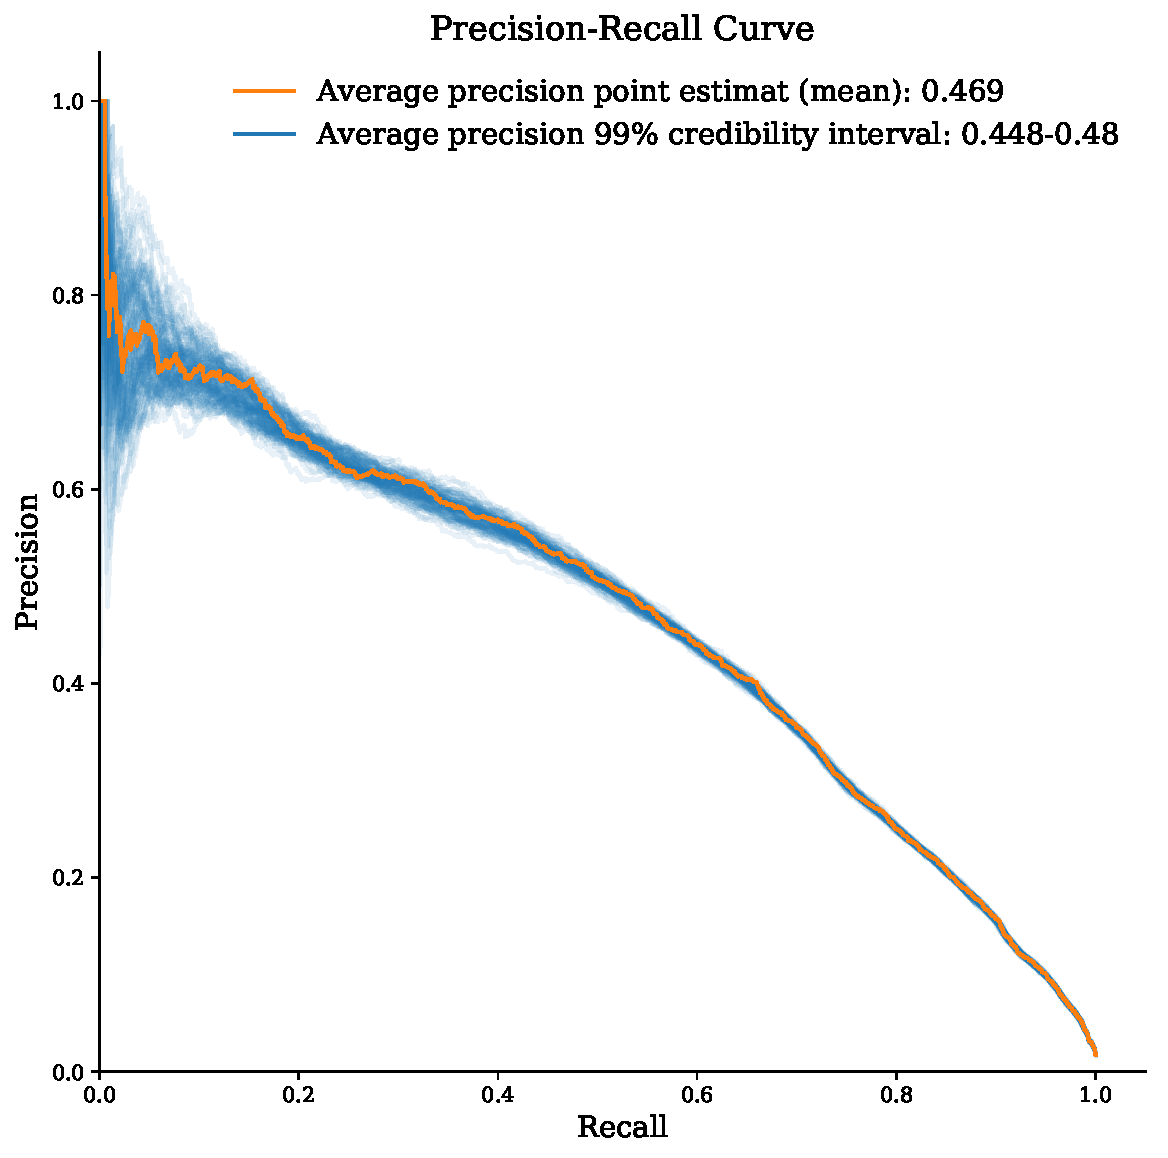
\includegraphics[scale=0.5]{pr_curve.pdf}
    \caption{\footnotesize{The credibility interval is plotted using only 100 random models for computational efficiency and no substantial changes comes from using all 1000. The reported credibility interval are based on all 1000 models. The point estimate (mean) reported and visualized are both derived on basis of all 1000 models}}\label{recall_precision_curve}
\end{figure}


The same information presented in \autoref{recall_precision_curve} is conveyed in \autoref{threshold_plot}, here merely at different specific marginal thresholds.\par

\begin{figure}[!htb]
	\centering
	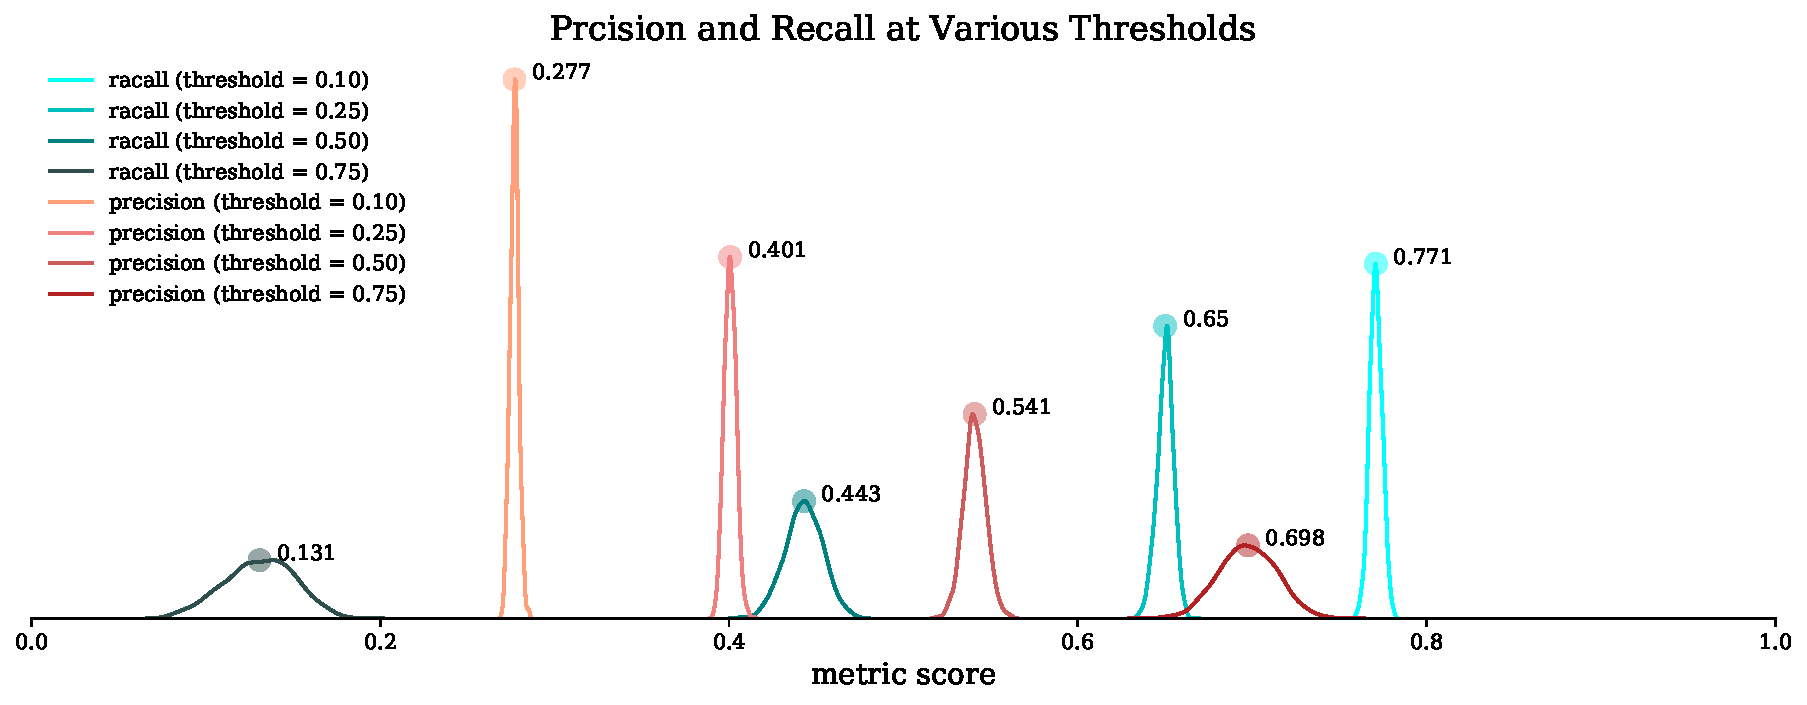
\includegraphics[scale=0.5]{threshold_plot.pdf}
    \caption{\footnotesize{Marginal distributions of recall and precision at various thresholds. The point estimate is marked and annoted while the specific threshold is given in the legend. The distributions are based on all 1000 xgboost models. As these sampling distributions can be interpreted as probability distributions the height of these does not convey any other meaning then the certainty pertaining to the estimates.}}\label{threshold_plot}
\end{figure}

Again, the inverse relationship and the increased variance with higher thresholds, is apparent. Furthermore, this plot gives us some substantial answers. For example; if we where to set a threshold denoting any PRIO grid with a probability of conflict above 10\% as a potential conflict zone, we would correctly identify 77.1\% of next years present conflicts. The trade-of is that these correctly identified events only constitute 27.7\% of the events predicted to have above 10\% risk of conflict. That is; our framework here generates around two false positives for each true positive. Or put another way; given this threshold, each time we predict conflicts in three cells, it is likely to only manifest in one them. But we would correctly capture almost 80\% of all conflicts.\par

Now, it is worth remembering that the grid cells in question are relatively small and does not correspond to any salient political, cultural or geographical distinction. It is merely squares. The point I am making here is, that predicting the exact cell is a vary hard case, and we can hardly hope to know exactly which of three neighbouring cells with high risk of conflict will actually experience conflict. And even if one experience conflict and the others do not, it does not mean that the risk was not real in all three cells. To illustrate my point \autoref{true_conf} illustrate all conflicts observed in 2007 versus the predicted probabilities for the same year in \autoref{pred_conf_b}.\par

\begin{figure}[!htb]
  \centering
  \begin{minipage}[b]{1\textwidth}
    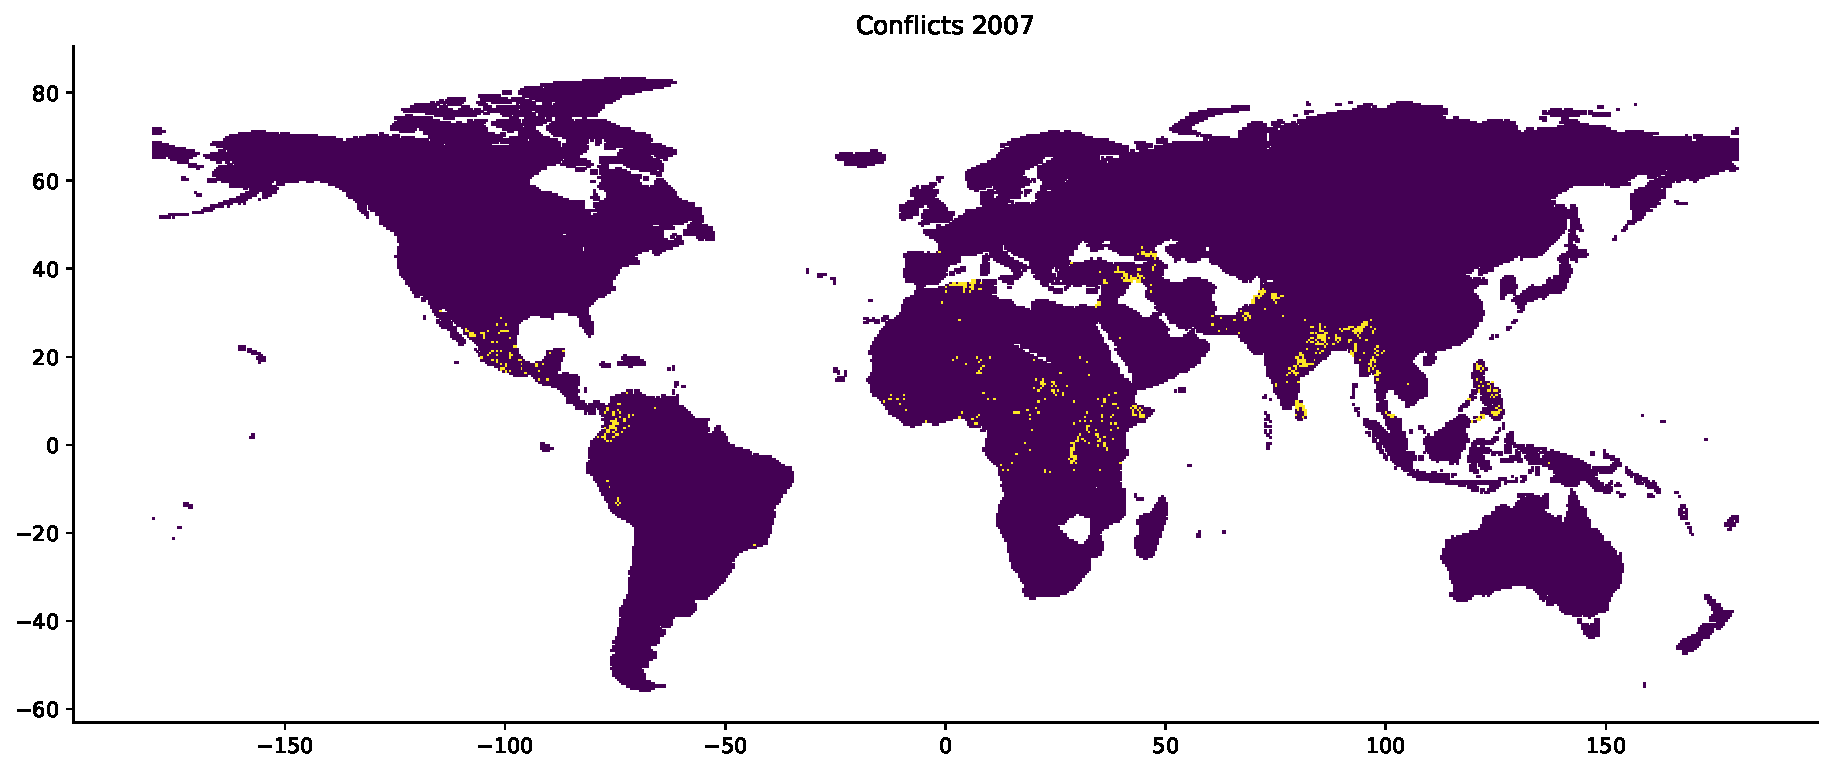
\includegraphics[width=\textwidth]{conflicts_2007.pdf}
    \caption{\footnotesize{Conflicts observed in 2007 by UCDP aggregated at PRIO grid cell level. The measure is binary, with yellow denoting one or more conflicts in the given cell. Afghanistan, Iraq, Turkmenistan, Georgia and Zimbabwe are missing due to the coding rules of UCDP.}}\label{true_conf}
  \end{minipage}
  \\	
  \begin{minipage}[b]{1\textwidth}
    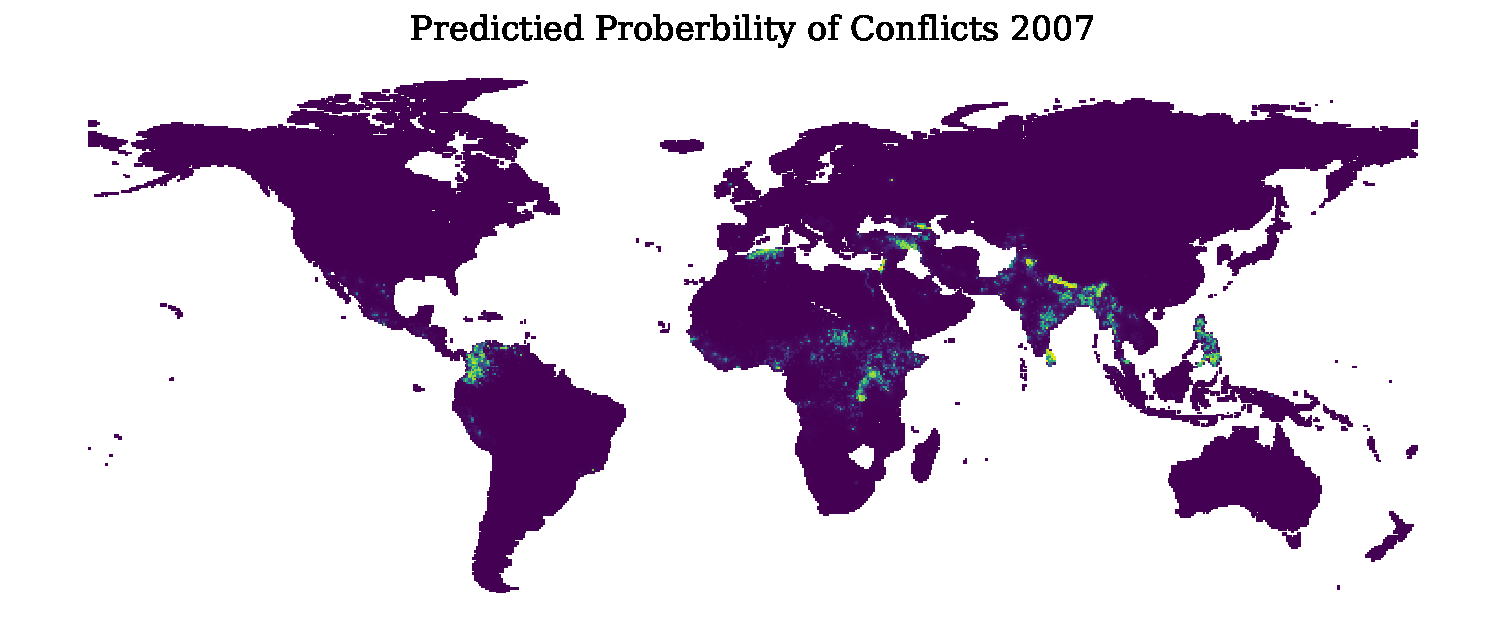
\includegraphics[width=\textwidth]{pred_prob_conflicts_2007_bayes.pdf}
    \caption{\footnotesize{The estimate probability (prior corrected) of conflicts in 2007 using data from 2006 and the model trained on data from 1990 through 2005. The measure is between 0 and 1, where a 1 would denote certain conflict and be colored bright yellow as in \autoref{true_conf}. Afghanistan, Iraq, Turkmenistan, Georgia and Zimbabwe are missing due to the coding rules of UCDP.}}\label{pred_conf_b}
  \end{minipage}
\end{figure}

The maps presented in \autoref{true_conf} and \autoref{pred_conf_b} clearly illustrates the potential of the framework - but also some of its challenges. It is clear to see that, for the most part, the areas deemed most probable of experiencing conflict, were also generally where conflict ensued. Indeed the predicted risk zones encompasses larger areas than the actual conflict zones, but this merely captures the uncertainty inherent in the task; we can hardly expect to know all the exact determinants separating which high risk zones actually end up experiencing conflict and which do not.\par

This is the good news. More problematic are the systematic mistakes. Looking at the year 2007 as an illustrative example, the high predicted probability of conflicts throughout Nepal constitutes a clear mistake; there was no conflict deaths in Nepal in 2007. Indeed, there where many conflict deaths from 1996 to 2006 as a result of the Nepalese Civil war \citep{ohchr2012nepal}, but non in 2007. The mistake is a product of the predictive framework - or indeed my construction of the framework. I ask my framework to present the probability of conflicts given the features presented earlier and that is what it does. However, none of the included features are able to capture sudden peace agreements or ceasefires - which is exactly what happened on 21th of November 2006 in Nepal \citep{ohchr2012nepal}. Thus, what my model is presenting is at best a counter factual statement; the probability of conflict across Nepal in 2007, if indeed the peace accord had not been concluded. The point is, that the framework is insensitive to sudden changes and developments in the political processes surrounding the conflicts and the sentiment among the warring parties. As I will discuss further down, this is crucial insight going forward towards a more accurate framework. However, before we come to that, the following section further explores why the framework is doing well in many instances, but also why it fails in e.g. the Nepalese case. This is done by analyzing which features the framework relies most heavily on generation its predictions.\par

% on nepal: \todo[inline]{du nævner også det her oppe i din indledning et sted - peg tilbage på det, bind en lille krølle - undervisere er vilde med den slags}

\subsection{Feature Importance}

Looking at the top five most important features in \autoref{feature_imp_plot}, four are directly related to present or past conflicts. Furthermore, the feature denoting distance to nearest conflict is by far the most influential predictor. More theoretical features pertaining to the greed versus grievance debate did not contribute with much prediction power once we included features modeling the temporal/spatial conflict pattern in it self. Intuitively this might not be surprising, yet the conventional literature, regarding prediction and parameter estimation alike, appears more occupied with scrutinizing greed and grievance related features, than modelling the pattern of conflict dispersion through time and space. To be sure, the literature does sometimes include measures of temporal/spatial dependency and dispersion, but these measures are often crude, ad hoc and theoretically underdeveloped - in which regard the present endeavour is no different. Naturally, I shall return to this matter in the discussion of future improvements.\par

\begin{figure}[!htb]
	\centering
	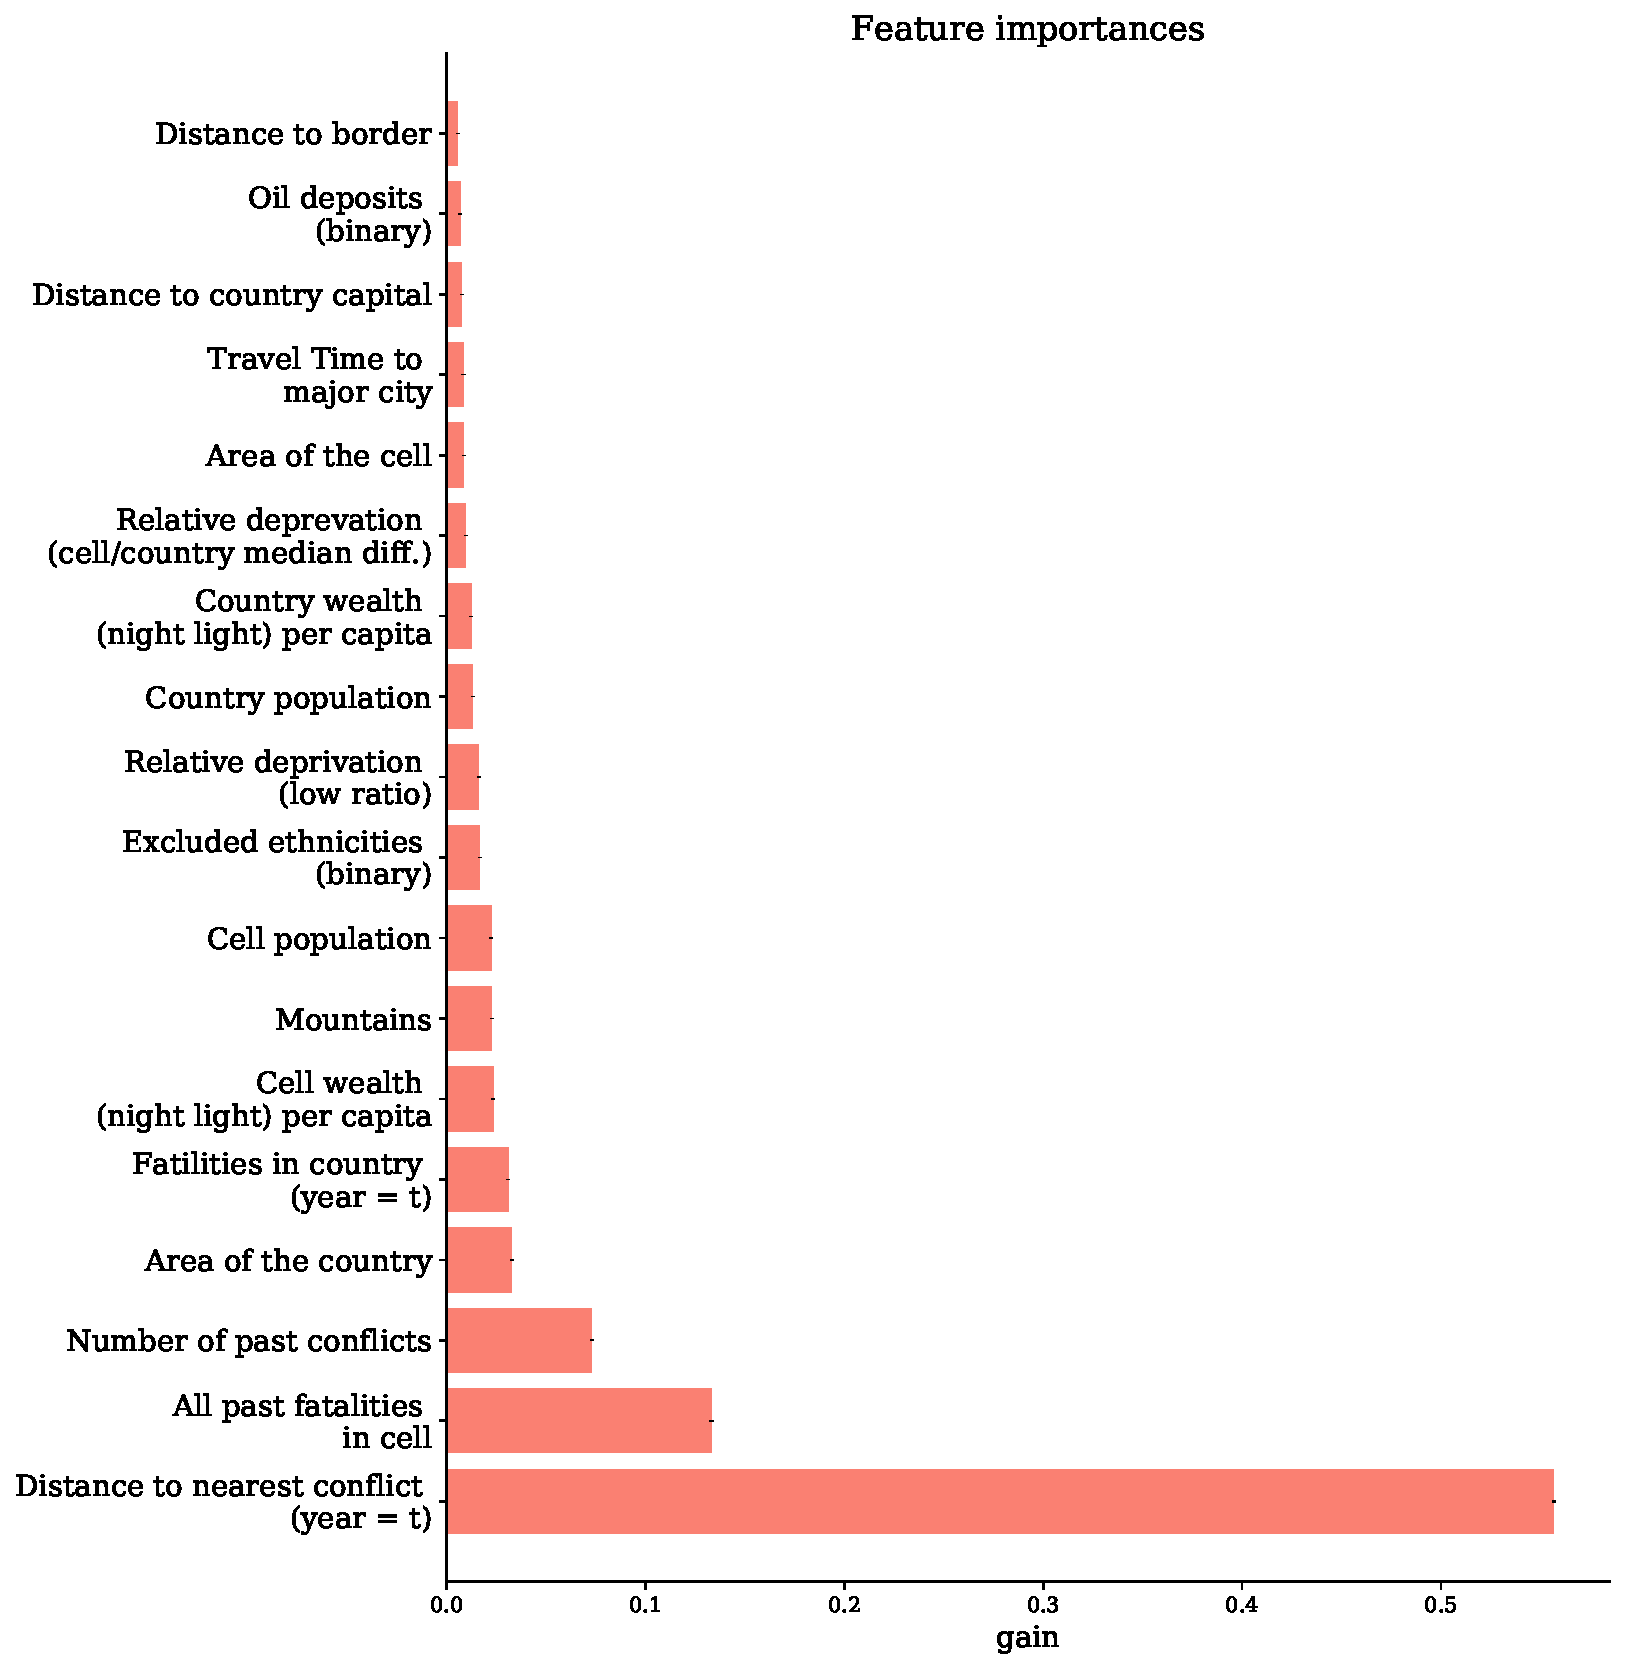
\includegraphics[scale=0.5]{feature_imp.pdf}
    \caption{\footnotesize{The relative importance of the included features given the use of the xgboost algorithm. Information from all 1000 models included. "Gain" denotes the internal optimization metric which the xgboost algorithm utilizes when choosing where best to split the generated regression tress.}}\label{feature_imp_plot}
\end{figure}

The question regarding Nepal is also neatly answered be the results in \autoref{feature_imp_plot}. As mentioned above, the framework gets almost all of its predictive power through past and present conflict patterns. To capture political events such as peace treaties we would need to include an altogether different type of features; features able of capturing sudden changes in the political development and sentiment in the given region or country. From this we can also deduce that the framework would be hard pressed, if it where to predict conflict onsets far removed in time or space from any other conflicts. Indeed a robustness test only including new conflict onsets, did perform markedly worse, but the hierarchy of feature importance did not change.\par

% Henvisning til appendix?

A proposal regarding handling of this issue is naturally presented in the discussion, to which I turn to now.\par

\section{Future Challenges and Improvements}

Having assessed the predictive capabilities of the framework I find three obvious avenues for improvement: an even better handling of the imbalanced data; a better, unified approach to the temporal/spatial inertia and dispersion of conflict; and the inclusion of features capturing more sudden political developments. These three avenues will be discussed in turn in the following subsections, after which I proceed to the summative conclusion.

\subsection{Balancing the Future}
An initial test showed that the framework did much better if the test data had been balanced in accordance with the train data. Naturally, such a test is only possible because we do have the actual conflict data of the test-set; which of course does not match any practical real world scenario. We could, however, take some precautions. For one thing, we know from the proceeding section that the best predictors are related to the temporal and spatial proximity of past and present conflicts. Thus, if New Zealand where to experience conflict next year do to some very unforeseen development, the framework would most likely not be able to capture it. With this in mind we could weed out all countries which have never experienced any conflicts in our data sample and which are also relatively far from any ongoing conflicts. This would, with all probability, reduce the number of non-events substantially, thus making the incoming data less imbalanced. Since we would not expect the framework to capture any conflict onset in the disregarded grid cells anyway, the trade-off might be negligible.\par

An other similar solution would be a "zero-inflated" framework with two or more rounds of estimations. The first round would correspond with the present endeavour. The second round would only include cells with a predicted probability over some appropriately low minimum threshold of conflict risk e.g. 1\%. This is more computational burdensome than simply sorting by country, but it is also more systematical and potential more powerful.\par  

\subsection{A Unified Temporal-Spatial Approach}

Temporal and spatial dependency, inertia and dispersion can be modeled in countless ways. Concerning the temporal dimension, most efforts have included some sort of fixed, random or conditional effects, but also more cleaver modeling of "conflict traps" and "conflict induced grievances" \citep{Collier_Hoeffler_2004, Hegre_Sambanis_2006, Cederman_Gleditsch_Buhaug_2013, perry_2013}. While these efforts are commendable, they all appear as ad hoc solutions. An example is \cite{perry_2013} who propose "time deteriorating index" where one would include the number of fatalities for each of the last ten years as features. The trick is then to down-weigh the fatalities by dividing with the number of years past since the corresponding events. Thus, a feature pertaining to fatalities two years ago will have, as its values, half of the fatalities observed that year\cite[14]{perry_2013}. While the heart of this proposal is at the right place, it is ad hoc and both methodologically and theoretically underdeveloped. There is no real reason to cap the effort at ten years. Even more, there is no theoretical or practical reason to choose the suggested deterioration rate. Instead of dividing with years past it might be more appropriate to multiply by 0.8 or 0.4; or the deterioration rate might have an altogether different functional form, like an exponential decay function. The point is that we do not know, and therefor we should estimate the function and not guess. Also, estimation at least gives us an indication of how bad our guess is. Intriguingly, estimation would also allow different regions, countries or cells to have different rates of conflict deterioration. I shall not go into the technical details here, but the machine learning technique of Gaussian Processes have been used to similar purpose with good results before \citep{Gelman_2013, Mcelreath_2018}. Furthermore Gaussian Processes also facilitates forecasting more readily, without the need to construct specific lags or leads in various features, as done in the present project. Again, it is hard to go into specifics without being technical, which would in turn demand a far greater reach than this written product allows, but in such a framework one could decide, post-modeling, whether one wanted estimates for next year, the year after or ten years ahead. Even more, the procedure also estimates the uncertainty which inherently grows as we look into the future.\par
 
Turning to the spatial aspect, I conveniently find that the same tools also have shown very good results in regards to spatial dispersion, where both regional and country\footnote{Or indeed any other geographical unit} specific variation again is readily incorporated \citep{gelfand2003spatial, gelfand2012hierarchical, gelfand2016spatial}. The fact that both the temporal and spatial patterns have potential of being modelled according to a unified approach is both practical and encouraging.\par

To clarify, I do \emph{not} propose to swap the xgboost algorithm, used above, with a new machine learning algorithm; I am suggesting that one could use the proposed techniques to create better features pertaining to the temporal and spatial patterns of conflict. Features which then could be fed some framework utilizing xgboost.\par

A less technical, but just as important point, is that modelling conflicts as a spatial/temporal function of conflict itself only requires the UCDP\footnote{Or any other relevant data source on conflicts} conflict data. As motioned in the beginning of this endeavour the UCPD data is substantially more up-to-date compared to the PRIO grid data. And indeed structural data such as that presented in the PRIO database are rarely available for the most resent years whatever the source. Thus, having learned that our model gets most of its predictive power from the UCPD itself, it seems only natural that any future effort to explore the potential in predicting conflict, considers using this database as the primary feature-source.\par

However, while I do believe such approaches holds great promise for future endeavours, they would not amend the challenge exemplified by Nepal 2007. The next subsection will present a potential solution to this shortcoming.\par

\subsection{Large Scale Automated Text Analysis}

The most simple and straight forward way to know whether some ceasefire is underway, is to know whether or not the warring parties are discussing a ceasefire. And furthermore whether or not the public and political sentiment appears to favour a potential ceasefire. To have this knowledge, regarding one specific country, is trivial. To have this knowledge regarding all countries collected as processable data, regularly and reliably updated, is an effort; but it is not impossible. Tools and approaches for large scale automated text analysis gets evermore accessible and powerful. And specifically automated text analysis utilized on online news sources have already shown promise in tasks of conflict prediction \citep{chadefaux_2014, mueller_2016}. 

Thus, one could enhance the feature-space with information pertaining to the political or public sentiment in various countries or regions by scraping large amounts of text data from social media, news sources or political outlets. Not only would such features potentially amend the problem exemplified by Nepal 2007; more importantly it could help in predicting onsets in otherwise peacefully areas \cite{mueller_2016}. As such, a framework incorporating analysis of text from news sources, social media and political outlets would bring valuable new information to the prediction effort.\par

The tread-of is naturally that such an effort is vastly more resource demanding than the two other remedies proposed. The amount of data needed to be process would be staggering. And even with access to ample resources one might be able to obtain country-specific information, but more disaggregated data would be a non-trivial task to obtain. Never-the-less, \cite{mueller_2016} show one way to do it, and with the pace of the present technological development it is surely not an impossible task.\par 

This concludes the discussion regarding future improvements of the framework. The following section will summarize the endeavors main points and conclude on the project as a whole.\par

\section{Conclusion}

The present endeavour was structured around three research questions, which have all been answered in turn. To reiterate:

\paragraph{$Q_1$:} Using a collection of modern machine learning tools I have explored to what extent is it possible to predict the geographic location of future intra-state conflicts. This was a preliminary endeavour, yet the results are quite encouraging. Indeed the framework does seem to successfully identify a larger proportion of high risk areas correctly. However, this is not without some imprecision. Thus, if we where to classify all predictions with a risk of conflict above 10\% as potential conflicts, we would correctly identify almost 80\% of all conflicts. However, given the imprecision of the framework, we would also produce two false positives for each true positive. However, many of these false positives are closely adjacent to actual conflict zones, and the thus, despite the lack of manifested conflict, the predicted risk might not be vastly overestimated. What is entirely more problematic is that the framework proves unable to capture sudden political events such as peace agreements or conflicts onsets far removed in time or space from any other conflicts. This leads us to the conclusion pertaining the second research question.\par

\paragraph{$Q_2$:} The sources of the frameworks strength is also the source of its weakness. The framework gets most of its predictive capabilities through features pertaining to the temporal and spatial patterns of past and presents conflicts. These features proved remarkable reliable in the prediction effort. But naturally a framework mainly relying on these dimensions will not be able to incorporate the effects of sudden political developments as described above. This leads us to the question of future improvements.\par 

\paragraph{$Q_3$:} Three proposals where given regarding future improvements. The first involves a better handling of the imbalanced nature of the data by disregarding countries which are deemed to have a very low probability of conflicts pre-estimation. Initial tests indicated that this could lower the trade-of between false negatives and false positives substantially.\par

The second proposed improvement involves creating a more unified framework for creating features pertaining to the temporal and spatial patterns of conflicts utilizing only the conflict data. Since these where the most informative dimensions, resources should be prioritized developing this avenue. Furthermore, this data is more fine grained; goes further back in time; are more often updated; and more up-to-date than the structural and contextual data used in the present endeavour. Thus altogether more suited for forecasting.\par

While these two improvements would no doubt improve the framework, they would not effectively handle the problem posed by sudden political developments. This, however, is the point of the third proposed improvement which would entail scrapping of country or region specific news sources or political outlets. This data could be analyzed using large scaled automated text analysis. Such endeavours have already been shown to capture sentiments and trends which holds predictive power pertaining to conflicts. While this would be a powerful addition to the framework, it is also vastly more resource demanding then the other proposed improvements.\par

With these recommendations regarding future endeavours, and a confident - if cautious - optimism regarding the prospect of a reliable early-warning-system the present project is concluded.\par

\pagebreak

\section{Bibliography}
\bibliographystyle{apalike} 
\bibliography{conflict.bib}

\pagebreak
\section{Appendices}

All python scripts used for the present endeavour are attach as HTML files or can be found on : \hyperlink{https://github.com/Polichinel/Conflict_Prediction}{https://github.com/Polichinel/Conflict\_Prediction}

The scripts are: interpolation.html, Feature\_eng.html, data\_exploration.html, div.html, C\_shapes\_lookup.html, boosting.html and evaluation.html  

\subsection{The Data Sources}\label{data_sources} % -------------------------------------------------------------------------

The project at hand utilize two different data source. The he Uppsala Conflict Data Program (UCDP) \citep{Sundberg_2013, Croicu_Sundberg_2017} and the PRIO grid\citep{Tollefsen_2012}. The first subsection below presents the UCDP while the follow presents the PRIO grid database.\par

\subsubsection{UCDP}

Most central to the endeavour at hand lies - of course - the data regarding intra-state conflict itself. This data is obtained through the Uppsala Conflict Data Program (UCDP) \citep{Sundberg_2013, Croicu_Sundberg_2017}. Specifically I utilize the UCDP Georeferenced Event Dataset (GED) Global version 18.1 \citep{UCDP_2017}. The dataset contains records of conflict fatalities and the corresponding coordinates. As mentions I utilized data from 1990 through 2010 but data from 1989 through 2017 is available in the database\footnote{For a smaller less detailed feature space data is available going back through 1975}. Conflict fatalities are here defined as: 

\begin{displayquote}

\emph{"An incident where armed force was used by an organized actor against another organized actor, or against civilians, resulting in at least 1 direct death at a specific location and a specific date."}\citep[38]{Croicu_Sundberg_2017}.

\end{displayquote}

Further definitions regarding armed force, organized actor ect. can be found in \cite[10-11]{Croicu_Sundberg_2017}.\par 

The project at hand limits itself to intra-state conflict, thus I only included incidents which do \emph{not} include two different nations as the organized actors\footnote{Naturally the distinction between a intra-state conflict and a proxy war can be very hard to uphold in practise. Never-the-less, though proxy wars are effectively between two states, the phenomenon is arguable more similar to intra-state conflicts and civil wars then to all out open warfare between to nations}. This data source provides the prediction target; the presence of conflict deaths in some geographic location in some future point in time. The data from UCDP is very detailed in regards to both temporal and spatial location, however for the endeavour at hand I aggregate the time unites to 'years' and the spatial resolution to the $0.5\times0.5$ decimal degrees grid cells provided by the PRIO grid. The target is further 'leaded' such that I am predicting conflicts one year into the future. Thus the prediction target is a binary feature denoting whether or not a given PRIO grid cell will host one or more conflict incidence the following year.\par

As I will show later on, many of the most important predictive features are also derive from this data source; e.g. the distance from a specific cell to the nearest conflict and the number of previous conflicts in a given cell. The fact that conflict patterns do them selves hold a lot of prediction power regarding future conflict zones might not surprise the reader, but I find the implications of this insight rather consequential in regards to future improvement of the framework, which I shall return to in the discussion.\par

\subsubsection{PRIO}

Given the geo-referenced nature of the UCDP data, the number of interesting data sources one could enhance it with are virtually endless. However, the aggregation of various geo-referenced and geo-spatial data accompanied with the appropriate grid construction and feature engineering can be a time consuming endeavour. While it is certainly a interesting and most likely fruitfully undertaking, it is one which will be saved for less preliminary work then the project at hand. Conveniently the Peace Research Institute Oslo (PRIO) has created what they call a "unified spatial data structure" \cite[1]{Tollefsen_2012}. More specifically they have divided the world - excluding Greenland and Antarctica - into grid cells of $0.5 \times 0.5$ decimal degrees. For each cell PRIO has gather a large selection of features, including economic, geographic and demographic features \citep{Tollefsen_2012}. Naturally the PRIO grid also extent itself across time, and the most current data includes cell-years from 1946 to 2015 - with some divergence in the data coverage across the years \citep{Tollefsen_2016}. On one side more complete data is available for more recent years; especially after 1990. On the other side no or little data is avialbel for the most recent years. Thus I utilize data from 1990 through 2010. This data includes relatively few random missing observations which are mainly handled through forward interpolation if possible, else backward interpolation or nearest observation. Some variables are only account for in 5-years intervals. This is handled through cell-specific linear interpolation as illustrated and described in the script \emph{interpolation.html}.

The PRIO grid is constructed as geo-spatial data and primed for collaboration with the UCDP data. As such merging and handling these two data source is a trivial task. For now I refrain from the temptation to included all variables available through the PRIO grid data base, and instead chose handpick features which are most often and constantly associated with internal conflict in the corresponding litterateur. There are number of reasons for this choice, but mainly it is to keep the endeavour concise, facilitate convertibility and due to the fact that initial tests indicated that few theoretically sound features outperformed the inclusion of many crude features. The following section will present the included features and also discuss some notable absentees.\par

\subsection{The Included Features - Expanded}\label{feature_expanded}

Below I give a spend some more ink on the theoretical backdrop support many of the included features. I also included some mathematical definitions where needed.

\subsubsection{Wealth and State Capacities}

 Easily one of the most robust findings in country level studies of civil wars is GDP per capita\footnote{Often logged and adjusted for purchasing power parity (ppp)} has a negative effect on the probability of civil war onset \citep{Collier_Hoeffler_1998, Fearon_Laitin_2003, Collier_Hoeffler_2004, Hegre_Sambanis_2006, Blattman_Miguel_2010} and also to some extent the conflict duration\citep{Fearon_2004, Hegre_Oestby_Raleigh_2009}.\par
 
 A number of mechanisms have been proposed linking GDP to conflict, Two have been especial prolific. The first is championed by \cite{Collier_Hoeffler_1998, Collier_Hoeffler_2004} sees GDP per capita as a proxy for opportunity-cost. that is what i given citizen have to loss by engaging in conflict. The second story draws on some insight from \cite{Skocpol_1979} and also echoes the gospel of modernization theory \citep{Lipset_1959}. Regarding the context at hand it has most prominently been presented by \cite{Fearon_Laitin_2003}. Here GDP per capita is seen as as proxy for state capacities. Simple put; weak or fragile states have low GDP per capita and these states are more conflict prone\citep[88]{Fearon_Laitin_2003}.\par
 
 A measure for GCP (Gross cell product) per capita (ppp) is included in the PRIO GRID from the Gecon dataset \citep{Nordhaus_2006} and this measure could be aggregated creating a feature for GDP per capita (ppp) \citep{prio_code_2015}. However the data available from the directly from the PRIO GRID only extent to 2010. Fortunately \cite{Elvidge_2009}, \cite{Chen_Nordhuas_2011} have shown that Night light emission can serve as an proxy for economic activities - especially for countries of areas with low-quality statistical systems and few or no recent population or economic censuses. \citep{Chen_Nordhuas_2011} - an approach explicitly proposed by \cite[p. 101]{Cederman_Gleditsch_Buhaug_2013} in regards to conflict studies. A ad hoc illustration of the high correlation between the two features can also be found in the script \emph{data_exploration.html}.\par
 
 The measure of Nigth Light Emmision in the PRIO GRID is borrowed from \cite{Elvidge_2014}it extent all the way up to 2015 and calibrated as to better accommodate time series \cite{prio_code_2015}.\par
 
 Just as the case with GDP ir GCP, it makes intuativly sens to correct the measure \emph{per capita}.
 
 \begin{itemize}
     \item $\frac{Cell-year specific Night Light Emission (mean)}{Cell population}$
     \item $\frac{Country-year specific Night Light Emission (aggregated mean)}{Country population}$ 
     %\item Country-year specific Night Light Emission (aggregated country median) % why? Den har du jo mest fordi du bruger den til at construere en anden var..
 \end{itemize}

Logged, density and measures not corrected for population size was also tired, but I found these measures less effective.\par

Naturrally one could argue that wealth is a relative concept, which leads us to the next section.\par

\subsubsection{Inequality and Deprivation} % ------------------------------------------------------------------------

If we - for the time being - leave the Strong State proposition behind and focus on the satisfaction of the individual citizens it is only natural to argues this satisfaction should be considered a function of \emph{what we have} and \emph{what we believe we rightfully should have}. This, indeed, is the crux of Robert Gurr's \citeyearpar{Gurr_1970} Relative Deprivation Theory. Perhaps one of the most seminal\footnote{At least after Marx} takes on inequality and conflict, \cite{Gurr_1970} defines relative deprivation: 

\begin{displayquote}
\emph{"[...] as actor's perception of discrepancy between their value expectation and their value capabilities. Values expectation are the goods and conditions of life to which people believe they are rightfully entitled. Value capabilities are the goods and conditions they think they are capable of getting and keeping."} \citep[24]{Gurr_1970}. 
\end{displayquote}

While intuitively appalling, Gurr's theory was award little credit doing the haydays of comparative corss country conflict studies. Supporting statistical results failed to materialize, and the axplanation eccoed the of \cite[11]{Skocpol_1979}; injustice and misery is simply to widespread to account for the rarity of major conflicts (\citealp[p. 22]{Collier_Hoeffler_1998},  \citealp[p. 22]{Collier_Hoeffler_2004} \citealp[p. 44]{Fearon_Laitin_2003}(FLERE?)). (så lige styr på de 22 side tal der?)

However, \cite{Cederman_Gleditsch_2009,Cederman_Gleditsch_Buhaug_2013} have noted that the aggregated country level features conventional used as indicators for inequality might lead to mis-specifications; that is, they do not properly measure the theoretical concept of relative deprivation or the correct mechanisms through which inequality affects conflict-propensity \citep[XX]{Cederman_Gleditsch_Buhaug_2013}. Acknowledging this critique I utilized the operationalization put forth in \cite[p. 104-105]{Cederman_Gleditsch_Buhaug_2013}\footnote{These scholars alos argues the higher conflict propensity might be fund in the other end of the inequality spectrum. That is; one could imagine a mechanism akin to relative deprivation in one end, while simultaneous at the other end, one might see well-off people wanting to secede from or take over a country if they fear to much redistribution. However, they find little statistical backing for this proposition, neither did my initial tests. Thus I only use the measures corresponding to actual Relative Deprivation}:\par

$$y_g = \textrm{country year mean}\quad ,\quad  y_c = \textrm{cell year value}$$
$$\textrm{low\_ratio} = y_c/y_g  \quad \textrm{if} \quad y_c < y_g, \quad 1 \quad \textrm{otherwise}$$

Thus cells which are relatively well of compared to the mean of country takes the value 1. Cells worse of the the country mean takes a value above 1, with the magnitude of this value indicating \emph{how} severe the deprivatione is. \cite{Cederman_Gleditsch_Buhaug_2013} Uses GCP per capita (ppp) but as mentioned also suggests using night light emission, Thus I here produce ratio feature solely on Night Light emission (cell-year mean).\par

While I do appreciate this operationalization I also construct my own relative deprivation feature, which differs in a number of small but relevant ways. First we know that wealth distributions in general are highly skewed, and this is no different when we use Nigt Light Emission as indicator. Thus, given Gurr's original conceptualization I find it more realistic that individuals should compare themselves to the median - not the mean. That is citizens in one cell compare their living standard to the most common living standard in the country over all. In the same vein, instead of a fraction, I simply calculate the difference between the cell-year values and the country-year median. Lastly I let the value start at 0. This I do to insure that interactions create later only "activates" if the cell is actually depraved. In the case of \cite{Cederman_Gleditsch_Buhaug_2013} when a cell is not depraved, the value of a interaction takes the naked value of the other interacted feature, which is arguably somewhat imprudent. Mathematical the features is formulated as such:\par

$$y_g = \textrm{country year median}\quad ,\quad  y_c = \textrm{cell year value}$$

$$\textrm{low\_diff\_median} = y_g - y_c  \quad \textrm{if} \quad y_c < y_g, \quad 0 \quad \textrm{otherwise}$$

Thus the feature takes the value 0 if the cell is on level or above with the rest of the country. If the cell is deprived the value correspond to the difference between the country-year median and the cell value. Naturally - and as we I shall return to later - this measure and the measure by \cite{Cederman_Weidmann_Gleditsch_2011} are highly correlated, nut that does not change the fact that this last feature appears somewhat closer to the notion of relative deprivation, and more impotently it handles interactions somewhat more appropriate or at least conventional. As before the feature uses on Night Light emission (cell-year mean) as indicator for wealth.\par

\subsubsection{Ethnicity and Exclusion}

Denotes the number of excluded ethnic groups (e.i. discriminated or powerless) in a given cell at a given year. The measures are originally from the GeoEPR/EPR data by \cite{Vogt_2015}. To better suit the theoretical argumentation laid forth in \cite{Cederman_Gleditsch_Buhaug_2013}(side) \citep{prio_code_2015}. I create a dummy (excluded\_binary) which simply denote \emph{if} there are any excluded ethnic groups. 

As with inequality the link between ethnic diverse societies and conflict propensity have been ridden with disagreement and controversies. In the quantitative literature results have remained somewhat inconsistent \citep[23-24]{Blattman_Miguel_2010}. A number of studies have fund different - and sometime quite convoluted - relationships between ethnicity or discrimination and conflict \citep{Collier_Hoeffler_1998, Fearon_2004, Blimes_2006, Hegre_Sambanis_2006, Goldstone_2010}, while other studies have fund little or no trace of the connection \citep{Fearon_Laitin_2003, Collier_Hoeffler_2004}(more? CH 2004 right?).\par 

As with the problem with inequality the lack of discernible results have often been attributed to poor feature specifications, a framework not capturing the proposed theoretical mechanism and not least country aggregated data \citep{Blimes_2006, Blattman_Miguel_2010, Cederman_Gleditsch_Buhaug_2013}. Mirroring they effort concerning inequality \cite{Cederman_Gleditsch_Buhaug_2013} have recently made use of new desegregated data \citep{Girardin_2015} to closer model the theoretical mechanism proposed. Without going to much in-depth here the feature \cite{Cederman_Gleditsch_Buhaug_2013} utilizes aims to capture the effect of \emph{horizontal inequalities} as defined by \citep[31-35]{Cederman_Gleditsch_Buhaug_2013}. That is the systematic discrimination or political exclusion of and coherent ethnic group. Thou not framed in the theoretical context of horizontal inequalities \cite{Goldstone_2010} finds results supporting the argument using the Minority at Risk data from \cite{Gurr_1995}.\par

Conveniently, a measure from \cite{Girardin_2015} of how many excluded ethnic groups reside in each PRIO GRID cell is readily aviable in the PRIO GRID. To mimic the theoretical proposition lead foth in \cite{Cederman_Gleditsch_Buhaug_2013} I binarize this variable to simply indicate whether or not a given cell is inhabited by a politicly excluded or discriminate ethnic group\footnote{Also initial test did not show much prospect of incorporating the full count}. 

Not surprisingly \cite{Cederman_Gleditsch_Buhaug_2013} futher finds that the properbilty of conflict gets even larger if political exclusion is followed by group deprivation, but the xgboost algorithm constructs it own interaction so I shall not be creating the interaction variable my self here.

\subsubsection{Population size and density} 

Returning to a variable with a rather flawless record regarding conflict onset we have "country population size" \citep{Collier_Hoeffler_1998, Fearon_Laitin_2003, Collier_Hoeffler_2004, Hegre_Sambanis_2006}\footnote{though see \cite{Goldstone_2010}}. Furthermore \cite[287]{Fearon_2004} also finds that country population is correlated with longer civil wars.\par

Lastly when it comes to disaggregated grid data, the "grid population size" also seems a rather robust predictor \citep{Buhaug_2010, Cederman_Gleditsch_Buhaug_2013}\footnote{Though see \cite{Hegre_Oestby_Raleigh_2009}}. Thus, whether the features influence conflict duration is more disputed \citep{Collier_Hoeffler_1998, Fearon_2004}. The most common implementation is to use a log transformed version of the country or grid population count\footnote{Though \cite{Collier_Hoeffler_1998} use the plain count in 10.000's} which is also implemented in the project at hand.\par

One very simple explanation might be the various definitions of conflict and civil war used throughout the litterature. These definitions almost always refer to some minimum fatalities count [eks and refs]. Naturally high population counts makes these threshold relativly less restrictive.\par

There are however also more theoretical propositions for the relationship. One being that conflict mediation becomes inherently more difficult as social systems and societies grow \cite[p- 271-272]{Diamond_1998}.\par

Initial I include features for cell-year population, aggregated country-year population and corresponding population densities:

$$\textrm{grid\_pop\_dens} = \frac{\textrm{grid\_pop}}{\textrm{grid\_area}}$$

$$\textrm{country\_pop\_dens} = \frac{\textrm{country\_pop}}{\textrm{country\_area}}$$

However, I find no gain to be made by including either the density or the logged count. Thus the raw count are utilized in the effort at hand.\par

\subsubsection{Geography and Accessibility} %------------------------------------------------------------------

\paragraph{Accessibility} As noted earlier, a strong state have often been presented as the prime inhibitor of internal conflicts. Naturally though, the strength of state must be considered relative to the territory over which it claims sovereignty - both in regards to size and permeability. \cite{Fearon_Laitin_2003} pointed to rough terrain and mountains as natural obstacles hindering effective projection of state power. Following this example \cite{Hegre_Sambanis_2006} concludes that a feature for rough terrain is found to robustly positively correlated with civil war across a large number of model specifications.\cite[526-529]{Hegre_Sambanis_2006}\footnote{Though see \cite{Goldstone_2010}}. The Prio Grid includes a readily available feature measuring the proportion of mountainous terrain within the cell based on \cite{Blyth_2002} wich I utilize.\par

Another natural hindering for projecting state power is sheer distance \citep{Fearon_2004, Buhaug_Gates_Lujala_2009, Cederman_Buhaug_Roed_2009, Buhaug_2010}. 

\begin{displayquote}

\emph{"The projection of power across distance comes at a cost. [...] In particular, large hinterlands and isolated peripheries are favorable to insurgency. In sum, this suggests that large countries are relatively more exposed to intrastate conflict"}\cite[113-114]{Buhaug_2010}

\end{displayquote}

A number of interesting features could be derived from Buhuag's assertion above (and the paper in general). What I have included is the distance to the nations capital\footnote{The measure utilized by \cite{Buhaug_2010}}, the travel time to the nearest major city, and the total size of the country\cite{prio_code_2015}.


\subsubsection{Trans-boarder Influences} %--------------------------------------------------------------------

A number of different mechanism have been proposed and explored \citep[29-30]{Blattman_Miguel_2010}, the one explored here is rather simple and follows \cite{Hegre_Sambanis_2006} I simply incorporate a measure for the distance to the nearest (land) border. I trued with the logged distance, but this yeilded no improvements. This is a very rough measure and is arguably a bit far removed from any specific theoretical concept, but for this preliminary project the measures will have to do.\par

\subsubsection{Prime Commodities and the Recourse course} %-----------------------------------------------------------

A lot have been written on this subject, but the empirical results have varied a lot \citep{Collier_Hoeffler_1998, Fearon_Laitin_2003, Fearon_2004, Ross_2004, Collier_Hoeffler_2004, Fearon_2005, Buhaug_2010, Hegre_Oestby_Raleigh_2009}. In this endeavour, I include a dichotomous feature denoting whether or not a given cell is known to hold oil deposits. Thus, a cell is not denoted as having oil before oil is actually discovered.\par

\subsubsection{Inertia, dispersion, traps and time trends} %---------------------------------------------------------------

Conflict traps and inertia have been modelled or proposed by many. \cite{Collier_Hoeffler_2004} uses a linear decay since last conflict; \cite{Hegre_Sambanis_2006} uses a linear decay since last peace; \cite{Cederman_Gleditsch_Buhaug_2013} count the number of previous conflicts; and \cite{perry_2013} propose a "deterioration index". Meanwhile, cross-country dispersion has been used by \cite{Goldstone_2010}. I include a number of features which aims to capture the pattern of conflict as it moves through space and time. Distance from cell center to nearest conflict, yearly fatalities in cell, yearly fatalities in the country as a whole and the total number of years the given cell has been a conflict zone in the past and .\par

\subsubsection{Notable Absentees}\label{notable_absentees} %---------------------------------------------

Notable missing include infant mortality, political system and intra elite conflict \citep{Goldstone_2010}. These should be tested in feature endeavours, but was not included here due to the limited scope of the project. The PRIO dataset did included a measure of infant mortality but it was ridden with missing values. Regarding the two other dimension, these would require the introduction of a third data source.\par

\subsubsection{Bayesian Prior Correction}\label{bayes_correction}

A small issue with the undersampling procedure above is that the probabilities predicted is somewhat inflated. This does not as such hurt the prediction effort. This might seem counter intuitively, but since the probability threshold beyond which we denote a observation to be a conflict can be chosen at will, it is the ratio between such threshold and the probabilities that. Not one or the other. To illustrate: normally one would set a threshold at 50\%. If the probability of conflict is above 50\% we predict a conflict and if it is below we do not predict a conflict. This threshold, while conventional, is entirely arbitrary and for some purposes it might well make more sense to set the threshold at 20\% or 80\%. Thus knowing that my estimates are inflated do to undersampling I could just easily set my threshold a bit higher then normal, say at 60 or even 80\%. However, I aim to not implement any hard threshold but instead presents the actual probabilities and their certainty for reader to survey. As such, for these probabilities to be intuitively meaningful they need to match what we actually know regarding the propensity of conflict events. This is easily implemented with an Bayesian prior correction\footnote{Related to what is presented in \cite{King_Zeng_2001, king_zeng_2001b} and \cite{Goldstone_2010}}. Denoting the the estimated probabilities of an event $Pr(E_{estimated})$, estimated probabilities of a non-event $Pr(NE_{estimated})$ the  and the corrected probabilities of events as $Pr(E_{corrected})$ the correction is as follows:

\[
Pr(E_{corrected}) = \frac{Pr(E_{estimated}) \times 0.2}{(Pr(E_{estimated}) \times 0.2)+(Pr(NE_{estimated} \times 0.8)} \tag{1} \label{eq:bayes}
\]

Where 0.2 is the prior, which is here set as the factor between the under sampled ratio of events of non-events and the actual ratio between events and non events. 0.8 is simply $1-prior$. The correction is a very crude utilization of Bayes theorem \citep[7-8]{Gelman_2013}, and could be much improved. Even more it is only semi-Bayesian since I use hard priors - scalars - instead of some appropriate distribution. A fruitful approach might also be to create cell, country or region specific priors possible in some hierarchical setting. This however is a challenge for an other endeavour. For now the crude correction will do - and as sown in \autoref{true_conf}, \autoref{} and \autoref{pred_conf_b} it does rather well. The point is that the non-corrected probabilities depicts a overly dangerous world. This can also be seen be setting an arbitrary threshold at 0.5 for classification. With the non-corrected probabilities this leads to a precision around 0.12 and a recall above 0.9, while the corrected probabilities splits it almost even. This proofs nothing, but it is a nice indication of more realistic estimates.\par

\begin{figure}[!htb]
  \centering
  \begin{minipage}[b]{1\textwidth}
    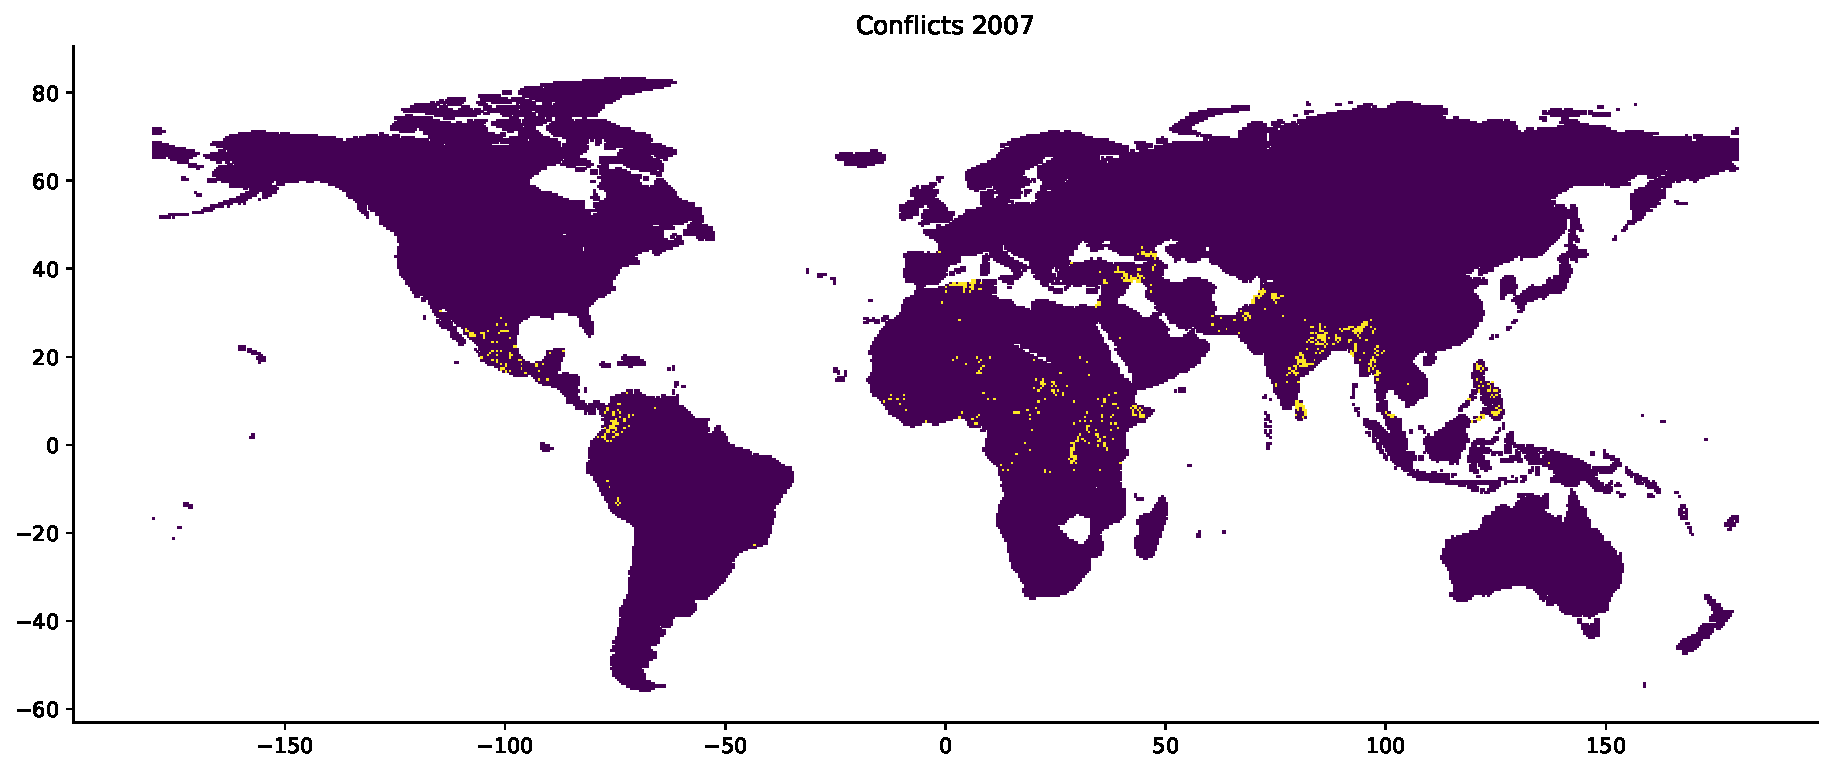
\includegraphics[width=\textwidth]{conflicts_2007.pdf}
    \caption{\footnotesize{Conflicts observed in 2007 by UCDP aggregated at PRIO grid cell level. The measure is binary, with yellow denoting one or more conflicts in the given cell. Afghanistan, Iraq, Turkmenistan, Georgia and Zimbabwe are missing due to the coding rules of UCDP.}}\label{true_conf}
  \end{minipage}
  \\	
  \begin{minipage}[b]{1\textwidth}
    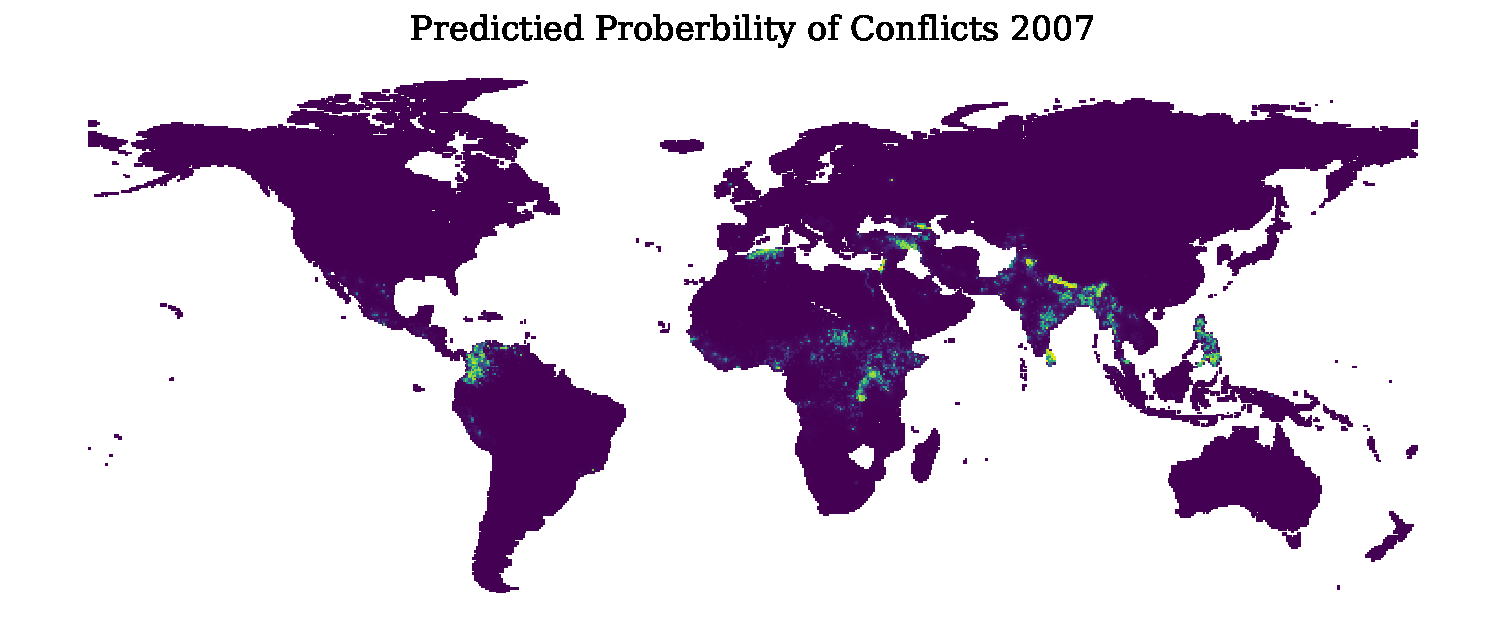
\includegraphics[width=\textwidth]{pred_prob_conflicts_2007_bayes.pdf}
    \caption{\footnotesize{The estimate probability (prior corrected) of conflicts in 2007 using data from 2006 and the model trained on data from 1990 through 2005. The measure is between 0 and 1, where a 1 would denote certain conflict and be colored bright yellow as in \autoref{true_conf}. Afghanistan, Iraq, Turkmenistan, Georgia and Zimbabwe are missing due to the coding rules of UCDP.}}\label{pred_conf_b}
  \end{minipage}
  \\
  \begin{minipage}[b]{1\textwidth}
    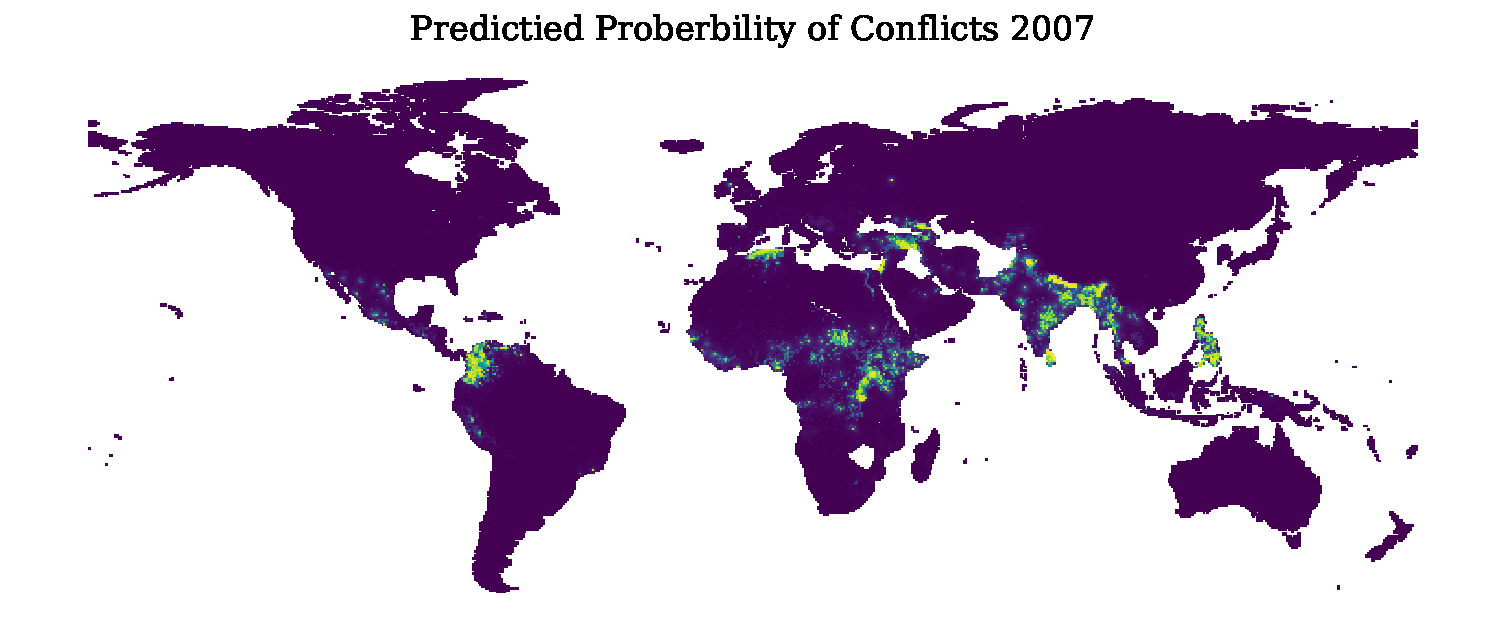
\includegraphics[width=\textwidth]{pred_prob_conflicts_2007.pdf}
    \caption{\footnotesize{The estimate probability (NOT prior corrected) of conflicts in 2007 using data from 2006 and the model trained on data from 1990 through 2005. The measure is between 0 and 1, where a 1 would denote certain conflict and be colored bright yellow as in \autoref{true_conf}. Afghanistan, Iraq, Turkmenistan, Georgia and Zimbabwe are missing due to the coding rules of UCDP.}}\label{pred_conf_b}
  \end{minipage}
\end{figure}

\end{document}
